\documentclass{article}

% If you're new to LaTeX, here's some short tutorials:
% https://www.overleaf.com/learn/latex/Learn_LaTeX_in_30_minutes
% https://en.wikibooks.org/wiki/LaTeX/Basics

% Formatting
\usepackage[utf8]{inputenc}
\usepackage[margin=1in]{geometry}
\usepackage[titletoc,title]{appendix}
\usepackage{float}

% Math
% https://www.overleaf.com/learn/latex/Mathematical_expressions
% https://en.wikibooks.org/wiki/LaTeX/Mathematics
\usepackage{amsmath,amsfonts,amssymb,mathtools}

% Images
% https://www.overleaf.com/learn/latex/Inserting_Images
% https://en.wikibooks.org/wiki/LaTeX/Floats,_Figures_and_Captions
\usepackage{graphicx,float}

% Tables
% https://www.overleaf.com/learn/latex/Tables
% https://en.wikibooks.org/wiki/LaTeX/Tables

% Algorithms
% https://www.overleaf.com/learn/latex/algorithms
% https://en.wikibooks.org/wiki/LaTeX/Algorithms
\usepackage[ruled,vlined]{algorithm2e}
\usepackage{algorithmic}

% Code syntax highlighting
% https://www.overleaf.com/learn/latex/Code_Highlighting_with_minted
%\usepackage{minted}
%\usemintedstyle{borland}

% References
% https://www.overleaf.com/learn/latex/Bibliography_management_in_LaTeX
% https://en.wikibooks.org/wiki/LaTeX/Bibliography_Management
\usepackage{biblatex}
\addbibresource{references.bib}

% Title content
\title{Ph237 Project 1: Gravitational Wave Astrophysics with White Dwarf Binaries}
\author{Xiang Li, Rico Lo, Shruti Maliakal, Jayce Miller, Yijun Wang, David Wu}
%\date{February 21, 2020}

\begin{document}

\maketitle

% Background and Introduction
\section{Aims of the project}

\begin{enumerate}
    \item A science case study
    \item Possibility with the existing / proposed detectors
\end{enumerate}

%  Main Body

\section{Background study}

\subsection*{Guide to the references}
\begin{itemize}
    \item For understanding the BWD population distribution \cite{Lamberts2019} has been the main resource, although it contains simulational and not observational evidence.
\end{itemize}


\subsection{PTA stuffs (Rico, David)}
%\cite{Hobbs2010} % This one is a good paper (we can 'copy' the structure of this review paper for our project)
Due to the stability of pulsars, simple models can predict pulse times-of-arrival (TOAs) with extreme precision ($<1 \mu s$) \cite{Hobbs2010}. Calculating timing residuals will shed light on GWs. Simply speaking, the simplest model for predicting the arrival time of future pulses from pulsars is 
\begin{equation}
    t=t_0+NP-\frac{1}{c}\hat{n}\cdot{\vec{D}}+R(t)
\end{equation}
where P is the pulsar period, N is the number of cycles the pulsar has undertaken since $t_0$, $\hat{n}$ is the unit vector pointing from the solar system barycenter to the pulsar, $\vec{D}$ is the vector pointing from the solar system barycenter to the telescope on earth, and $R(t)$ is GW contribution to the delay of arrival time as GW induces a fluctuation in the observed pulse frequency such that the residual timing is computed as
\begin{equation}
    R(t)=-\int_0^t\frac{\delta \nu}{\nu}dt=-\int_0^tH^{ij}\left[h_{ij}(t_e,x_e^i)-h_{ij}(t_e-D/c,x_p^i)\right]dt
\end{equation}
where $D$ is the distance between earth and the pulsar while $H^{ij}$ is a geometrical pre-factor depending on the alignment of the Earth, the pulsar and the GW source.) Using least-squares fitting (`Bayesian' or `frequentist' approaches are both valid here), intrinsic parameters of the pulsar, i.e. pulsar pulse period, spin-down (i.e. the change in pulse period), orbital motion, are then inferred. To know what signal caused the timing residuals, a search of correlation across multiple pulsars must be performed (this is to properly isolate out the effects purely caused by GW which is valid only after assuming an isotropic, stochastic GW background). (Some numbers on detecting GW using PTA: 20 pulsars timed with an r.m.s. timing residual of $\sim 100 \; {\rm ns}$ over 5 years with observations every week (i.e. abundance could really help solve this issue)).

Pulsars issues (timing irregularities): (a) irregular rotation rate; (b) low-frequency noises; (c) modeling errors. Note, these do not really matter much as we are interested in millisecond pulsars (PTAs) which are stable. But with this in mind, to really say we have detected GW, some pretty standard statistical procedures must be in place for the selection of pulsar timing data. (Note: GW is `detected' when we observe correlated timing residuals between different pairs of pulsars).

\subsection{\label{BWDgeneral}BWD general (Shruti, Yijun (Ali))}
While there does seem to be an abundance of Binary White Dwarfs (BWDs) in the Milky Way Galaxy ($10^{6}$ to $10^{7}$)  which will result in a large low frequency (0.1- 10 mHz) noise in the LISA bandwidth \cite{Farmer2003}, the GW signal from an individual binary would be $<1.15 \times 10^{-21}$  \cite{Lamberts2019} (assuming 1$M_\odot$, 1kpc and f=2 mHz). Comparing this to the sensitivity curve for LISA \cite{Hobson2018}, it is barely detectable. The 'galactic background' in Figure 1 of \cite{Hobbs2010} is representative of what we are looking for.

In order to be able to measure other GW signals as modulation over a stable single frequency GW emitted from a BWD, we must further be sensitive to even smaller modulations in this frequency. There would be an associated strain sensitivity curve for modulation GW signals \textit{for each BWD}. 
\cite{Farmer2003} mentions that the net background galactic BWD contribution can be subtracted due to its spatial anisotropy and the changes in this with the revolution of LISA in its orbit. This cannot be immediately applied to individual BWDs because the spatial resolution of LISA would most likely be insufficient.

Table 4.5 (and text below) of \cite{LISA1998} says that the angular resolution of LISA at $\sim$ 1 mHz would be $\sim$ 0.05 sr. An approximated value of the areal density of BWD population is 6200 /(kPc)$^2$ along the plane of the Milky Way (?). Therefore, within one `pixel' at 1 kPc distance there could be over hundreds of BWDs (For comparison, the diameter of the Milky Way is 32 kPc).

The evolution of the BWD GW signal frequency is (Equation 7 of \cite{Farmer2003}):
\begin{equation}\label{BWDfevol}
    \dot{\nu} \simeq (3.7 \times 10^{-6} s^{-2} (\mathcal{M}/M_{\odot})^{5/3}\nu^{11/3}
\end{equation}
So, for a BWD with 1 solar mass equivalent chirp mass $\mathcal{M}$, at 1 mHz, it would be $\sim37 \times 10^{-18}$  Hz/s or $\sim1$ nHz/year. (The limit to the frequency comes from the frequency resolution of LISA: a 1$M_\odot$ BWD's accumulated change in frequency over the LISA nominal lifetime (5yr) is just equal to the df resolution of LISA, estimated simply by 1/(5yr) In this regime, we can assume a constant intrinsic f, and any measurable df is due to GW modulations. Using the inverse of the equation above, we get around 2 mHz, assuming 1$M_\odot$). Note that this limit is not very sensitive to the change in mission time. If the mission time increases by a factor of 10, this frequency limit decrease only by a factor of 1.87.

\textbf{Further Work}
\begin{itemize}
    \item What is the general trend of the strain sensitivity of modulation on the BWD GW signal?
    \item How hard would it be to matched filter these modulations?
    \item Detection process modeling for continuous waves. Possibly useful paper on the analysis here: \cite{Schutz1997}.
    \item in addition to detector noise sensitivity level, which is the most dominant noise for burst signals, continuous wave signals have uncertainties associated with Doppler effects. Might be important when we calculate the detection threshold.
    \item work with the PTA formula and write out explicitly what the modulation is. From there we could proceed in two ways. Either we combine the WD strain and extragalactic sources information (typical freq, typical strain) and work out the required detector SNR, or we go in reverse; use WD strain and known SNR of certain detectors and work out what the required strain amplitude is for the extragalactic sources (here extragalactic sources refer to any low freq GW sources)

\end{itemize}

\begin{figure}[H]
    \centering
    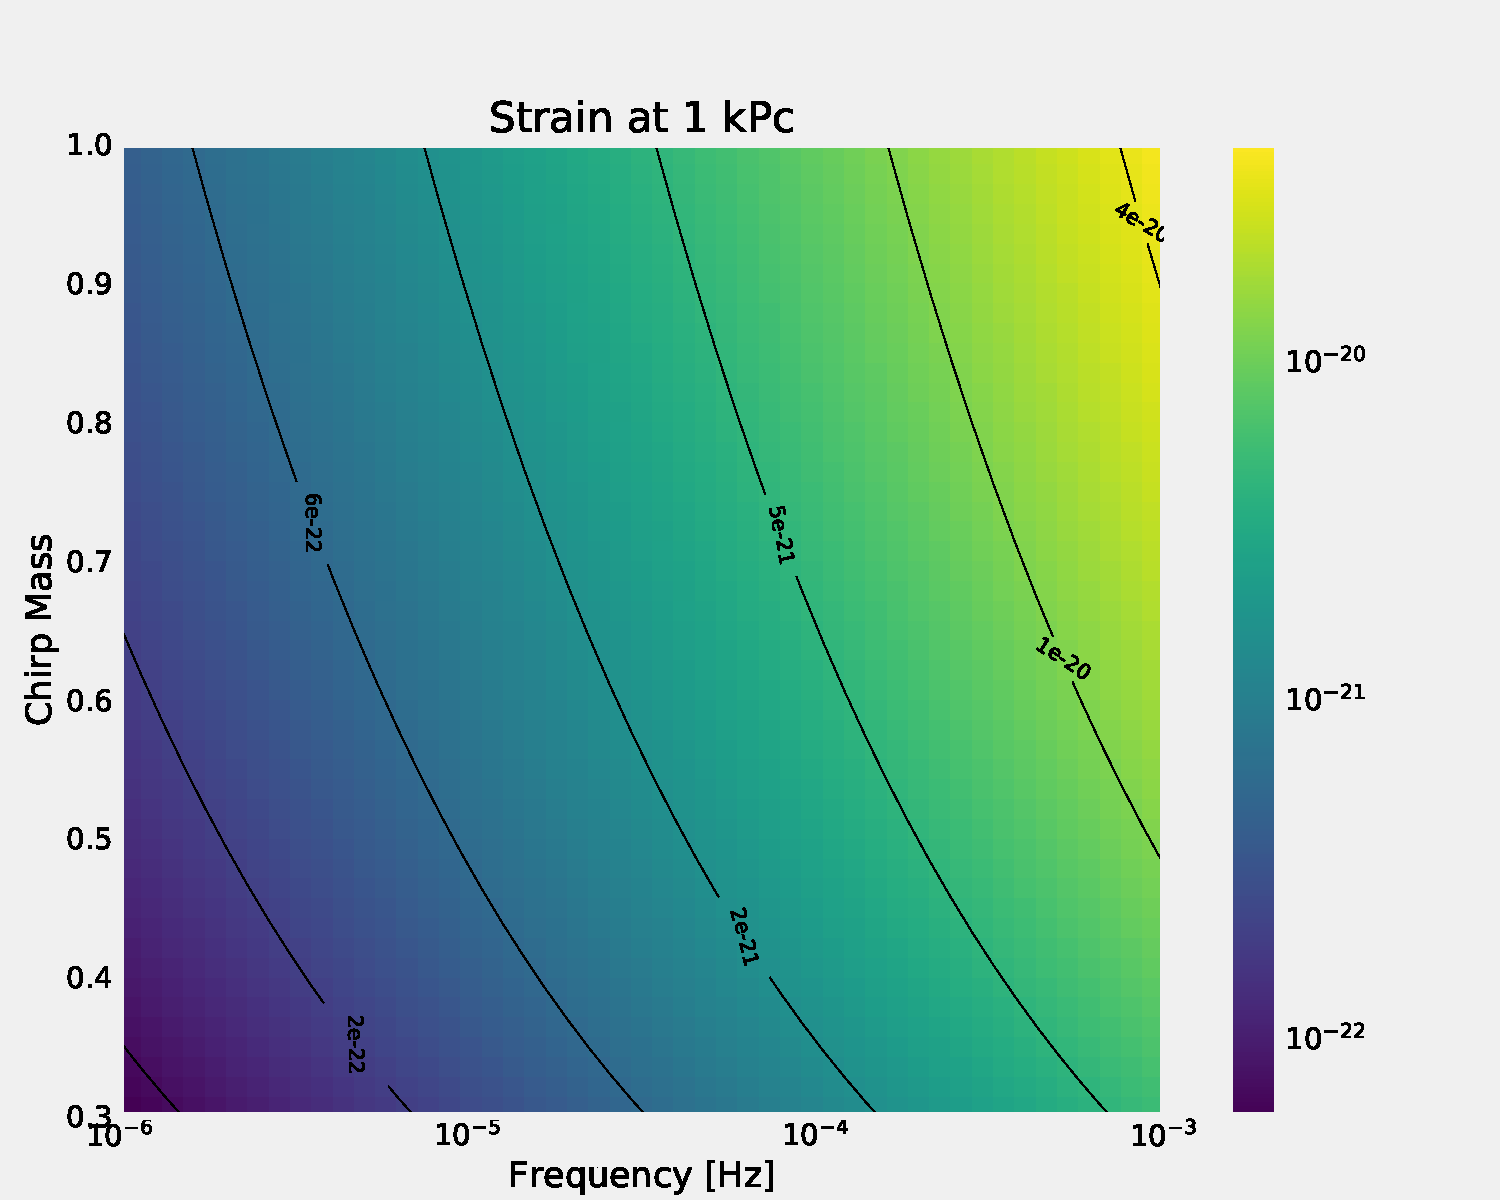
\includegraphics[width=10cm]{Strain1kpc.pdf}
    \caption{Estimated strain for BWD at 1 kiloparsec (quadrupole formula)}
    \label{fig:h1kpc}
\end{figure}

\begin{figure}
    \centering
    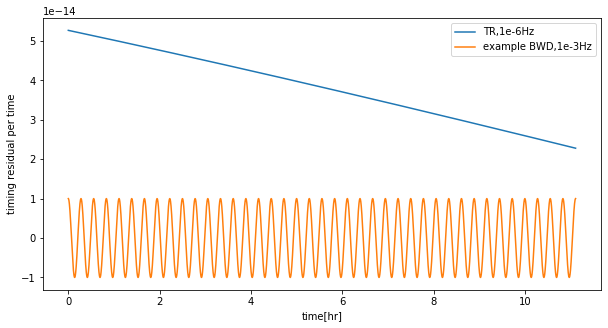
\includegraphics[scale=.6]{TR.png}
    \caption{Example fractional timing residual curve and example GW signal from BWD. The example source is a 1e8 Msun equal-mass binary at 1Mpc, emitting GW at 1e-6Hz. A sine curve with f=1e-3Hz is drawn to illustrate a BWD signal.}
    \label{TR1}
\end{figure}

\begin{figure}
    \centering
    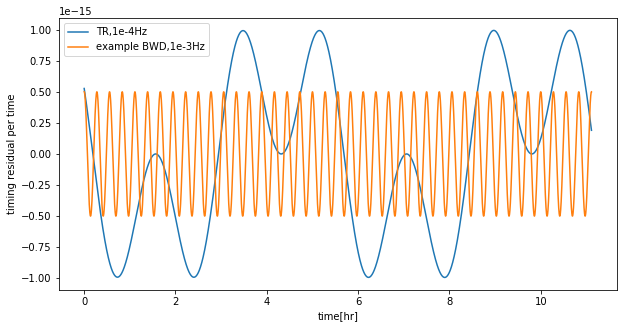
\includegraphics[scale=.6]{TR2.png}
    \caption{Similar plot to the figure above, but the gravitational wave frequency is 1e-4Hz (from an equal mass binary of 1e6 Msun at 1Mpc.}
    \label{TR2}
\end{figure}

Since these modulation varies much more slowly than the BWD, we can approximate their waveform as a constant over several cycles of BWD. Then we can directly use Eqn.1 and calculate the fractional timing residual. Then the change in the period is approximated by $R_{\rm{frac}}\Delta t$, through which we can get the new frequency as $f(t)=1/(T_0+R_{\rm{frac}}(t-T_0))$. Note that this is a crude leading order approximation, but this should be valid when the BWD frequency and that of the low-freq GW source are quite different. As they get closer, we might use further linear/quadratic expansions. 


\subsection{BWD as the GW probe (Xiang, Jayce)}

\subsubsection{Frequency band requirement}

The mass distribution of white dwarf is $0.17-1.33 M_\odot$, it peaked at $0.6 M_\odot$, and the majority lies between $0.5-0.7 M_\odot$\cite{Kepler2007}. We can assume the same mass distribution for BWD as a third of white dwarfs are in binary systems (WD+WD, WD+MS, etc.) \cite{Holberg2009}. Note the two extreme cases below: 

\begin{itemize}
    \item \textbf{ZTF J153932.16+502738.8} is a binary white dwarf with the shortest-ever-known orbital period of 6.91 minutes. (corresponding to the question in the previous section) Its period has been observed to be decreasing (?), due to the emission of gravitational waves. Its GW strain has frequency $4.8 mHz$ and amplitude $1.6 \times 10^{-22}$. We thus notice that the largest GW frequency of BWD is $4.8 mHz$.
    \item \textbf{Hen 2-428} is the most massive BWD system known (as of 2015). Its GW strain has frequency $0.14 mHz$ and amplitude $9.89425\times10^{-23}$.
\end{itemize}

Well, according to \url{http://gwplotter.com/}, it seems that LISA is hopeless in terms of strain sensitivity...

Let's assume the sensitivity of LISA (or some other detector) is enough at $mHz$ band. A valid detection has the following requirement:
\begin{enumerate}
    \item From PTA analogy\cite{Hobbs2010,Moore2015}, \emph{if the external GW frequency modulation mechanism (will discuss in Sec.\,\ref{theoretical}) is similar}, we can do detection for frequency at most one OoM smaller than the probe. Most BWD lies below $mHz$ band, thus the max frequency we can detect is $10^{-4} Hz$. \emph{Is there any reason for PTA not being sensitive below $10^{-9}$?}
    \item We need at least a whole period to claim the observation of a smaller frequency signal. The designed lifetime for LISA is 4-5 years\cite{Lamberts2019}, thus $8\times10^{-9} Hz$ is the min frequency we can detect. \emph{We can not make a hundred-year-long detector -- can we?}
    \item To detect the frequency change caused bu external GW modulation apart from the intrinsic evolution estimated by Eq.\,\eqref{BWDfevol}: for a year long detection, we can not detect modulation frequency lower than $10^{-9}Hz$. \emph{Probably that DC change can be subtracted...but the detection is limited by the detector lifetime anyway.}
\end{enumerate}

In analogy to PTA case\,\cite{Moore2015}, viewing the BWD network as a Milky Way scale interferometer, we probably can not detect signal below $10^{-9}Hz$. Considering the difficulty for BWD localization analyzed in Sec.\,\ref{BWDgeneral}, there might be no advantage compared with PTA to detect sources below $10^{-8}Hz$. But a comparison from a different method will still be very interesting.

\subsubsection*{Signal integration}
For continuous wave signal, we might integrate for a long time $T$ to boost the SNR $\propto\sqrt{T}$ as the signal will add coherently (i.e. with a single frequency component) while the noise will add incoherently. 

LISA need at least $10^{-19}$ strain sensitivity in $10^{-4}-10^{-3}$ frequency band, where BWDs roughly have $10^{-22}$ strain. Thus, we need at least 2 weeks of integration to boost the SNR for 3 OoM. According to Eq.\,\eqref{BWDfevol}, the BWD GW frequency 
will drift about $4\times10^{-11}Hz$ in 2 weeks, which will not be a big issue. Because of the 2 weeks' integration time, the maximum sampling rate will be $8\times10^{-7}Hz$. Thus, according to Nyquist–Shannon sampling theorem, we can only reliably extract external GW signals lower than $4\times10^{-7}Hz$.

\subsubsection*{Timing residual and frequency}
Considering the BWD as an antenna and a background lower in frequency gravitational wave signal ($S_{fs}$) we want to measure. As a first order effect, assuming the signal is weak, the timing change in the orbital period ($T$) results in a frequency modulation of the measured GW frequency of BWD $f_{GW}$). Since we are integrating over multiple orbits, we have,
$$\frac{\Delta \omega}{\omega} = \frac{\Delta T}{T}$$
where $\Delta T(f)$ would have the same spectrum as $S_{fs}$.

If the signal can be approximated as continuous wave $\Delta T = hT\cos(2\pi f_s t)$, where t is sampled much more slowly than $T$ but faster than $1/f_s$. This would therefore result in a drifting frequency that depending on the choice of analysis could turn up as a bias in the estimation of $f_{GW}$.
$$\Delta f = hf_{GW}\cos(2\pi f_s t)$$

\subsubsection*{Doppler Shift and triangulation}
When using a detector such as LISA to observe the GW emission from a BWD even if the BWD emits solely because of its orbital motion, we would not simply measure $f_{GW}$.
\begin{enumerate}
    \item We would measure a Doppler shifted $f_GW$ due to the relative motion of the intra-galactic BWD and the detector, which to properly account for would require an accurate estimate of the relative velocity
    \item We would also see the effects of the evolution, which in order to account for would require an accurate estimate of the chirp mass and $f_{GW}$ itself
\end{enumerate}


\subsubsection*{Phase and amplitude modulation}
For phase modulation, there will be frequency drift in different sample points (as Rico plotted in his .ipynb). For amplitude modulation, there will be additional sidebands, which might be difficult to observe due to its low value.
(Shruti)I think we would probably just see changes in the amplitude of the signal at the BWD frequency if we are measuring at the same time-scale as before.

\subsubsection*{Conclusion}
 we should focus on sources in $4\times10^{-7}-8\times10^{-9} Hz$ frequency band. There can be cross-check with PTA method in $10^{-8}-10^{-9} Hz$ band.



\subsubsection{Sources}

The $10^{-4}-10^{-7} Hz$ frequency band is relatively blank. Perhaps some stochastic background and supermassive binaries not detectable by PTA on $10^{-5}-10^{-6} Hz$ bad?

\subsubsection{Other detectors}
TianGo?\cite{Kevin2019}

\subsubsection*{Things to be considered}

\begin{itemize}
    \item (added by Alvin Li) LISA sensitivity curve, and the expected ``confusion limit curve" :
    
    \begin{figure}[h!]
        \centering
        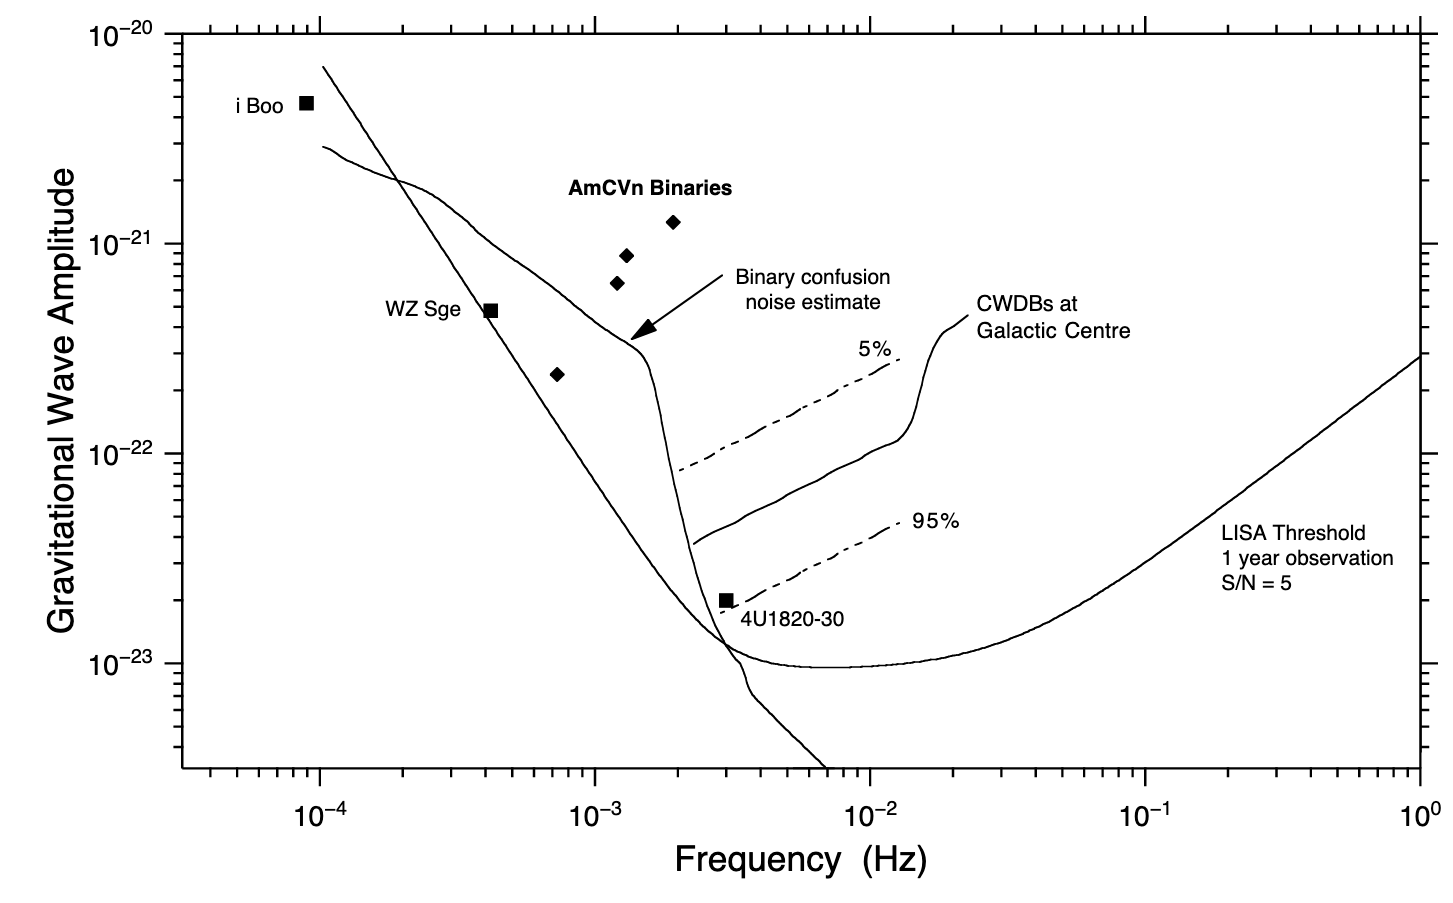
\includegraphics[width=0.7\textwidth]{LISA_sensitivity_curve.png}
        \caption{\label{fig:LISA_sensitivity} The sensitivity curve and the estimated binary confusion noise estimate.}
    \end{figure}
    
    \item A proposed idea (in 2019) of discovering exoplanets by measuring gravitational waves from BWD with exoplanets orbiting around: \url{ https://www.nature.com/articles/s41550-019-0807-y}. The effect of the orbiting exoplanet will be imprinted (causes modulation) to the gravitational waves from the BWD)

\end{itemize}

\section{BWD population in the Milky Way}
This section summarizes the literature review and analysis on the population distribution of BWDs in the Milky Way in terms of their mass, frequency, spatial distribution and other properties.

White dwarfs are remnant stars that sustain from collapse by electron degeneracy pressure. The upper limit to their mass is 1.4 M$_\odot$, given by the Chandrasekhar limit. 95\% of all stars become white dwarfs, and further, since two of these can become gravitationally bound by a common envelope phase to form a binary, a large number of such BWDs is also expected. These binaries can either be \textit{detached} (with no mass exchange) or \textit{interacting} (with tidal interaction and mass exchange). While interacting BWDs are easier to observe in EM, for our purpose as antenna for secondary GW sources, detached binaries are preferred due to it being easier to analyze gravitationally.

The first binary white dwarf (BWD) was observed in 1967 (cite) and the first detached BWD in 1988.

\begin{table}[h]
    \centering
    \begin{tabular}{c|c}
         &  \\
         & 
    \end{tabular}
    \caption{Modified from Table 1 of \cite{Lamberts2019}}
    \label{tab:lamberts}
\end{table}

\subsection{Population density and spatial distribution}
and Table 1 of \cite{Lamberts2019} 

\subsection{Mass distribution}
The upper limit to the mass of a single white dwarf being 1.4 M$_\odot$ 


\subsection{Frequency distribution}

\subsection{Peculiar velocities}

\section{Proposed works}

Make an analogy with PTA \cite{Moore2015}

\subsection{\label{theoretical}Theoretical: How BWD GW signal affected by smaller frequency GW?}

\begin{enumerate}
    \item Frequency modulation (perturbation on the detector near earch)
    \item nanoHz GW is ‘pumping’ energy to the BWD system? (perturbation on physical evolution of BWD)
\end{enumerate}


We can still start from the previously proposed timing residual calculation done for the PTA detection. Some key characteristics related to the pulsar signal such as distance to earth, $x_p$, $t_p$ etc. will now be adapted to the BWD data: $x_{bwd},t_{bwd},D_{bwd}$. Therefore, intuitively, we can direclty make the analogy and conclude that if using the residual timing method, we will obtain the following computation for the signal analysis of BWD: (Using Yanbei's notes for a more intuitive explanation)
\begin{align}
    R(t)&=-\int_0^t\frac{\delta v}{v}dt'=-\int_0^t H^{ij}\left[h_{ij}(t_e,x_e^i)-h_{ij}(t_e-D/cx_{bwd}^i)\right]dt'\\
    &=\int_0^t\frac{D}{2}\sum_p\frac{e^p_{jk}(N)n^jn^k}{1-n\cdot N}\left[h_p(t-N\cdot{x_e})-h_p(t-D-N\cdot{x_{bwd}})\right]dt
\end{align}
where we can clearly see the polarization of the strain and individual earth term and BWD term contribution to the residual timing.

As the notion of sensitivity of each detector is given in the frequency domain, we will need to simultaneously investigate the frequency domain of our residual time function. We can do this via Fourier transforming our expression from t-space to f-space:
\begin{equation}
    R(\omega)=-\int_{-\infty}^{\infty}\left(\int_0^tH^{ij}\left[h_{ij}(t_e,x_e^i)-h_{ij}(t_e-D/cx_{bwd}^i)\right]dt'\right)e^{-i\omega t}dt.
\end{equation}

\textbf{Some concerns:}
\begin{enumerate}
    \item Are BWDs as stable as millisecond pulsars? If not, what are the known sources of instability and can we incorporate these into our residual timing function by adjusting the arrival time of pulses from BWD accordingly?
    \item Are frequency modulations sufficient to detect GW parameter modulations, or do we need to strengthen our claim via amplitude modulation detection as well? 
    Amplitude modulations would be hard to detect unless we integrate long enough to observe the individual sidebands, assuming these signals last that long, or if we have sufficient strain resolution to detect changes in the amplitude.
\end{enumerate}

While we cannot eliminate the sources of unstable signal, i.e. noises in some cases, we can adapt the integration boosted SNR approach by allowing the detection to be carried out over a longer period (estimated 1 hour (LISA?) for BWD s.t. we can still obtain a clear signal in the range of $10^{-4}Hz\sim 10^{-7}Hz$ as discussed above) s.t. during this period, signal will add coherently and noise will add incoherently. Thus, greatly decreasing the effect of noise on our signals.



\subsection{Simulation:}

\begin{figure}[H]
    \centering
    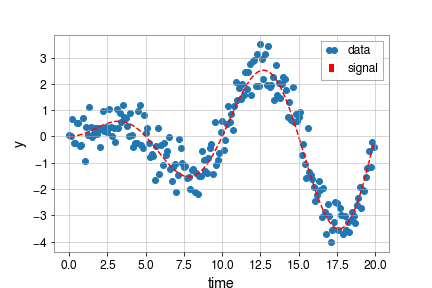
\includegraphics[width=6cm]{data.png}
    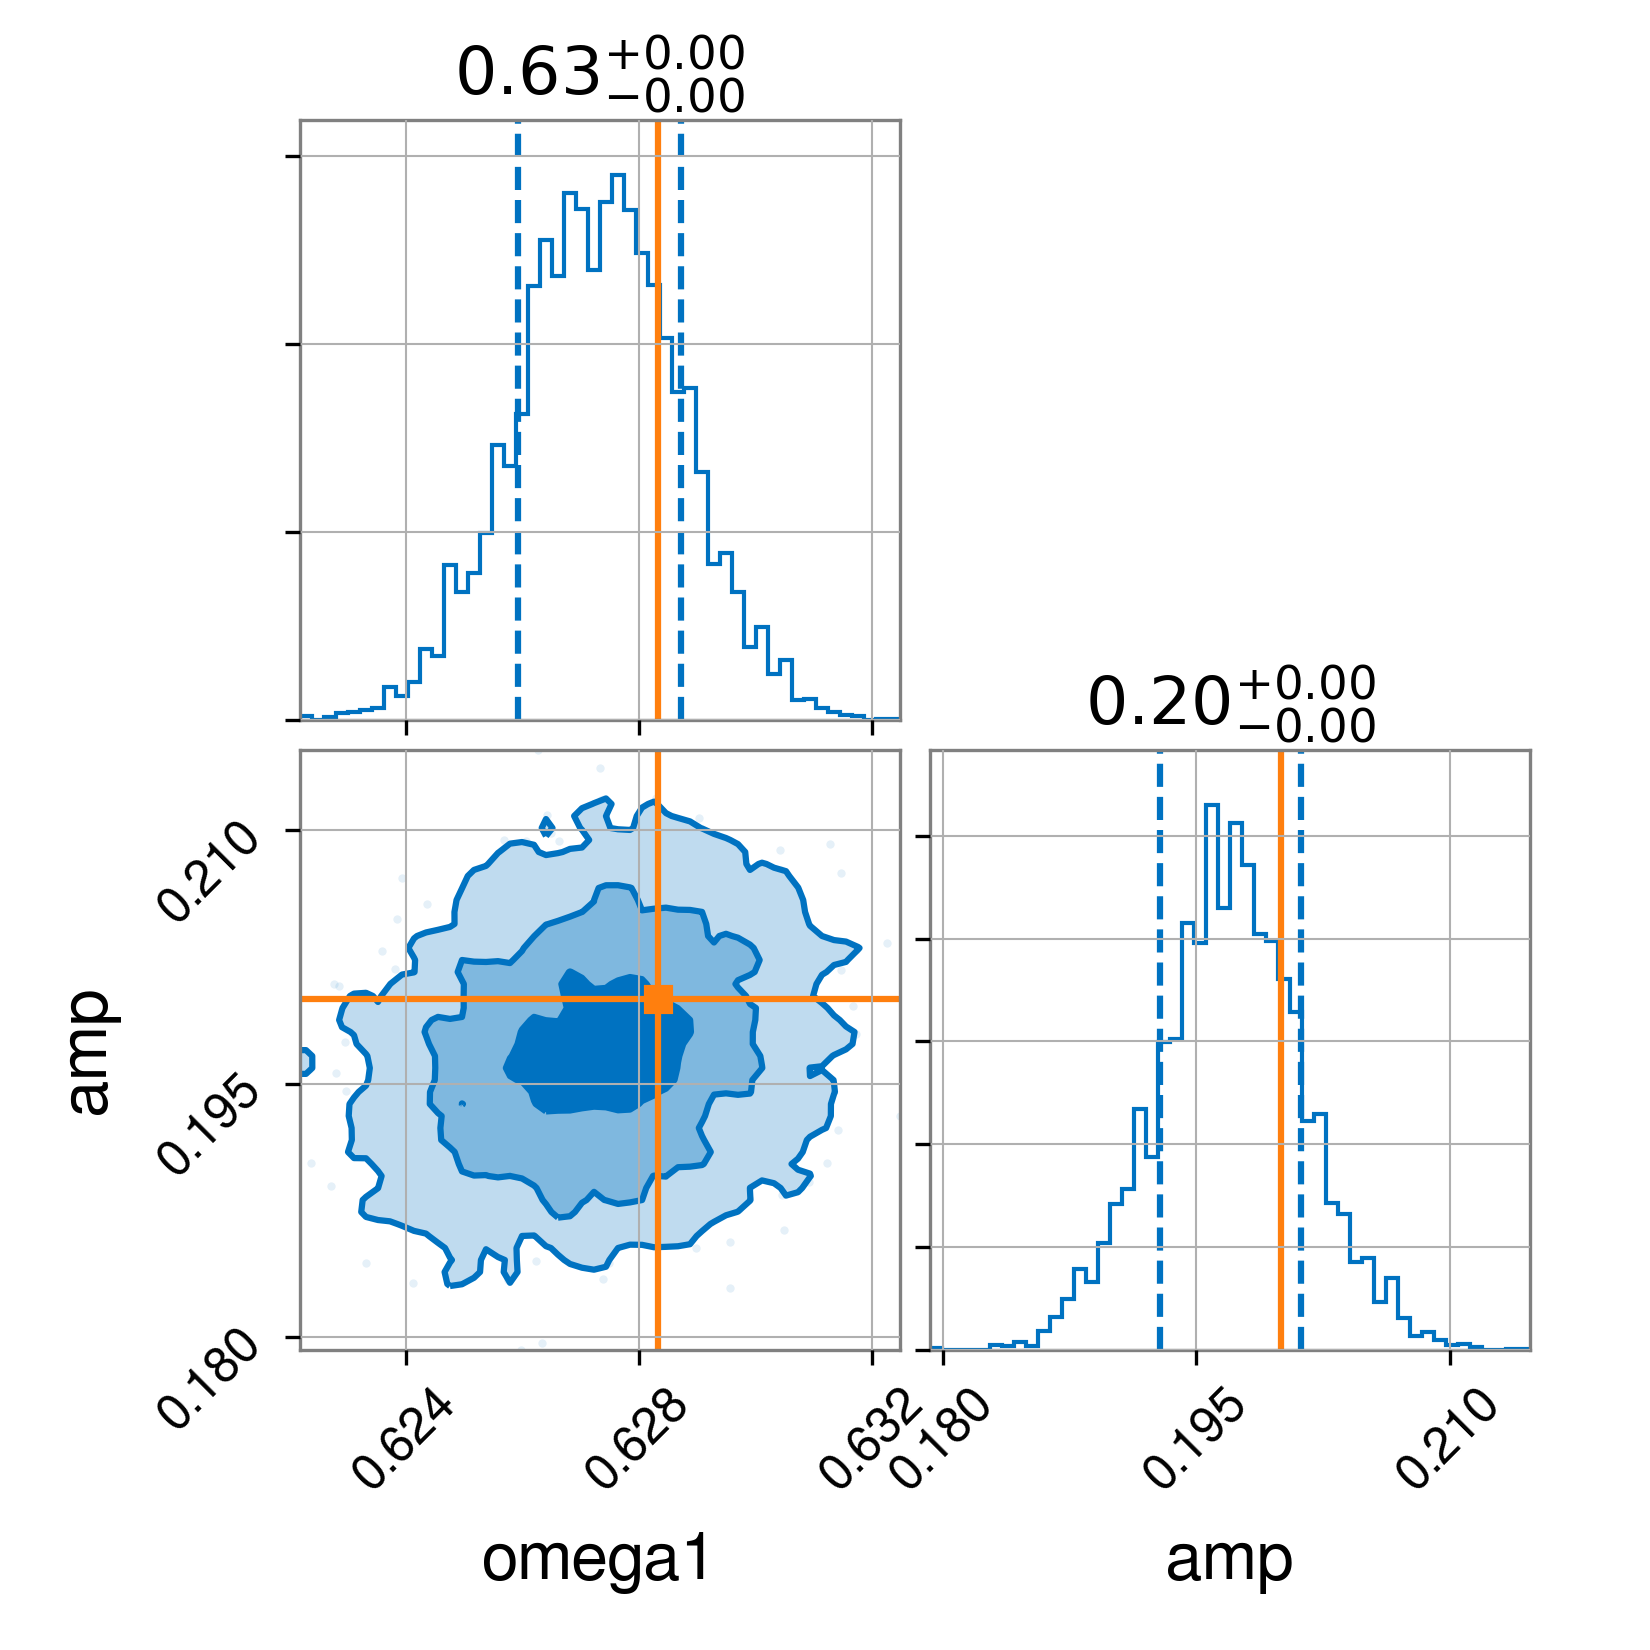
\includegraphics[width=6cm]{corner.png}
    \caption{Simulated data of phase residual}
    \label{fig:h1kpc}
\end{figure}

% References
\printbibliography

%\bibliography{references}
\end{document}
